\documentclass[border=6pt]{standalone}
\usepackage{tikz}
\usetikzlibrary{arrows.meta,positioning,calc,shapes.geometric}
\begin{document}
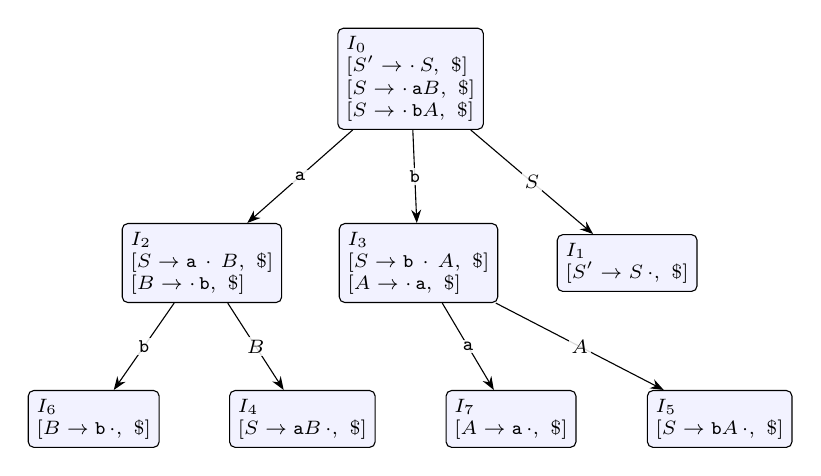
\begin{tikzpicture}[>=Stealth,font=\scriptsize,x=1.000cm,y=1.000cm,
 box/.style={draw,rounded corners=2pt,align=left,inner sep=3pt,fill=blue!5},
 circ/.style={draw,circle,align=center,inner sep=1pt,minimum size=0.75cm,fill=blue!5},
 lab/.style={font=\scriptsize,inner sep=1pt,fill=white,fill opacity=0.85,text opacity=1}]
\node[box] (s0) at (0.000,0.000) {\textbf{$I_{0}$}\\$[S' \to \cdot\,S,\ \$]$\\$[S \to \cdot\,\mathtt{a} B,\ \$]$\\$[S \to \cdot\,\mathtt{b} A,\ \$]$};
\node[box] (s1) at (-2.650,-2.340) {\textbf{$I_{2}$}\\$[S \to \mathtt{a}\,\cdot\,B,\ \$]$\\$[B \to \cdot\,\mathtt{b},\ \$]$};
\node[box] (s2) at (0.100,-2.340) {\textbf{$I_{3}$}\\$[S \to \mathtt{b}\,\cdot\,A,\ \$]$\\$[A \to \cdot\,\mathtt{a},\ \$]$};
\node[box] (s3) at (2.750,-2.340) {\textbf{$I_{1}$}\\$[S' \to S\,\cdot,\ \$]$};
\node[box] (s4) at (-4.025,-4.320) {\textbf{$I_{6}$}\\$[B \to \mathtt{b}\,\cdot,\ \$]$};
\node[box] (s5) at (-1.375,-4.320) {\textbf{$I_{4}$}\\$[S \to \mathtt{a} B\,\cdot,\ \$]$};
\node[box] (s6) at (1.275,-4.320) {\textbf{$I_{7}$}\\$[A \to \mathtt{a}\,\cdot,\ \$]$};
\node[box] (s7) at (3.925,-4.320) {\textbf{$I_{5}$}\\$[S \to \mathtt{b} A\,\cdot,\ \$]$};
\draw[->] (s0) -- node[lab,midway] {$\mathtt{a}$} (s1);
\draw[->] (s0) -- node[lab,midway] {$\mathtt{b}$} (s2);
\draw[->] (s0) -- node[lab,midway] {$S$} (s3);
\draw[->] (s1) -- node[lab,midway] {$\mathtt{b}$} (s4);
\draw[->] (s1) -- node[lab,midway] {$B$} (s5);
\draw[->] (s2) -- node[lab,midway] {$\mathtt{a}$} (s6);
\draw[->] (s2) -- node[lab,midway] {$A$} (s7);
\end{tikzpicture}
\end{document}
